% !TEX TS-program = pdflatexmk
% Load the rcclab class pass bibstyle=<style> to change biblatex style (chem-acs, chem-rsc, chem-angew, etc.)
\documentclass{rcclab}
% Head.tex includes useful packages and macros  
\usepackage[version=4]{mhchem} % Formula subscripts using \ce{}
\usepackage[separate-uncertainty=true]{siunitx}
\sisetup{detect-all}
\usepackage{enumerate}
\usepackage{xcolor}
\usepackage{color, colortbl}
\usepackage{subfig} % For sub figures because some people like them for some reason
\usepackage{xr} % For cross-referencing figures
\hypersetup{pdfauthor = {R.C. Chiechi et al},
pdftitle = {Manuscript for submission},
pdfsubject = {Manuscript for Submission},
pdfcreator = {LaTeX with hyperref package},
colorlinks, breaklinks, linkcolor=black, urlcolor=black, anchorcolor=black, citecolor=black
}

%
% BibLaTeX Setup
% Change options below for different publishers use \autocite{} in the tex files
%
\usepackage[utf8]{inputenc}
\usepackage[style=chem-acs]{biblatex}
\addbibresource{references.bib}
%
%

%%%%%%%%%%%%%%%%%%%%%%%%%%%%%%%%%%%%%%%%%%%%%%%%%%%%%%%%%%%%%%%%%%%%%
%% Place any additional macros here.  Please use \newcommand* where
%% possible, and avoid layout changing macros (which are not used
%% when typesetting).
%%%%%%%%%%%%%%%%%%%%%%%%%%%%%%%%%%%%%%%%%%%%%%%%%%%%%%%%%%%%%%%%%%%%%

\newcommand{\red}[1]{\textcolor{red}{#1}}
\newcommand{\blue}[1]{\textcolor{blue}{#1}}
\newcommand{\green}[1]{\textcolor{green}{#1}}
\newcommand*{\ie}{\textit{i.e.}, }
\newcommand*{\eg}{\textit{e.g.}, }

\newcommand*{\ts}[1]{$\mathrm{#1}^{\mathrm{TS}}$}
\newcommand*{\mica}[1]{$\mathrm{#1}^{\mathrm{Mica}}$}
\newcommand*{\cp}[1]{$\mathrm{#1}^{\mathrm{AFM}}$}

\newcommand*{\fermi}{E_\mathrm{f}} % Use inside math
\newcommand*{\egap}{E_\mathrm{g}} % Use inside math
\newcommand*{\Junits}{\si{Acm^{-2}}}
\newcommand*{\logJ}{$\log|J|$}
\newcommand*{\logI}{$\log|I|$}
\newcommand*{\vtrans}{$V_{\mathrm{trans}}$}
\newcommand*{\vtransp}[1]{$V_{\mathrm{trans}}^{#1}$}
\newcommand*{\degC}[1]{\SI{#1}{\celsius}}
\newcommand*{\et}{\textit{et al}.}

% Declare molar units with siunitx
\DeclareSIUnit\Molar{\textsc{M}}

% Examples of macros for defining molecule abbreviations
\newcommand*{\Tn}[1]{\textbf{C4T#1}}
\newcommand*{\TnC}{C4T\textit{n}}
\newcommand*{\Thn}{T\textit{n}}
\newcommand*{\OPEn}{OPE\textit{n}}
\newcommand*{\BDT}[1]{\textbf{BDT-#1}}

% Examples of custom macros for this paper
\newcommand*{\DTT}{\textbf{DTT}}     %DTT
\newcommand*{\dDTT}{\textbf{\textit{d}-DTT}}  %dimerised DTT
\newcommand*{\bpDTT}{\textbf{(bp)\textit{d}-DTT}}  %bidentate physisorbed DTT
\newcommand*{\mpDTT}{\textbf{(mp)\textit{d}-DTT}}  %monodentate physisorbed DTT
\newcommand*{\bcDTT}{\textbf{(bc)-DTT}}  %bidentate chemisorbed DTT
\newcommand*{\C}[1]{\textbf{C#1}}           %use as \C{0}, \C{1}, etc.
\newcommand*{\Cn}{\textbf{C\textit{n}}}     %lipoic acid, just use as \Cn
\newcommand*{\EtSH}{\textbf{EtSH}}     %Ethanethiol
\newcommand*{\AuS}{\textbf{Au--S}}     %Au-S bond
\newcommand*{\AuSS}{\textbf{Au$\dotsm$(S--S)}}     %Au--S-S bond
\newcommand*{\AuSSAu}{\textbf{Au$\dotsm$(S--S)$\dotsm$Au}}     %Au--S-S bond
\newcommand*{\SSbond}{\textbf{S--S}}     %S-S bond
\newcommand*{\AuSH}{\textbf{Au$\dotsm$SH--R}}     %Au-SH physisorbed bond
\newcommand*{\AuAu}{\textbf{Au--Au}}     %Au-Au bond
\newcommand*{\F}{figure}
\newcommand*{\m}[1]{\textbf{#1m}}     %S-S bond

% Place all Main Tex figures in the figures/ subdirectory
\graphicspath{{figures/}}
% Load supporting_information.aux to use cross-references
\externaldocument{supporting_information}
% authorlist.tex contains the list of authors
\title{A Succinct and Informative Title}

\author{First Author$^{1,2}$,% email
	    Second Author$^{1,2}$,% email
	    Third Author$^{1,2}$% email 
	    and Ryan C. Chiechi$^{*1,2}$% r.c.chiechi@rug.nl
}


% This is useful for debugging UTF-8 errors
%\DeclareUnicodeCharacter{0301}{*************************************}

%
% Begin the document
%
\begin{document}
% Render the title and authors
\maketitle
% affiliations.tex contains the affiliations for each author
\begin{affiliations}
 	\item Stratingh Institute for Chemistry, University of Groningen, Nijenborgh 4, 9747 AG Groningen, the Netherlands
 	\item Zernike Institute for Advanced Materials, Nijenborgh 4, 9747 AG Groningen, the Netherlands
	\item[] *e-mail: r.c.chiechi@rug.nl
\end{affiliations}
% Write an abstract
\begin{abstract}

A succinct abstract.

\end{abstract}

% Add some keywords
\textbf{Keywords:} Keyword 1, Keyword 2, Keyword 3, Keyword 4, Keyword 5

%
%Target Journal:
%

%% Outline
\begin{outline}

    \item What did you do?
    \begin{itemize}
        \item A descriptive sentence that may begin ``this paper describes\dots''.      
    \end{itemize}
    
    \item Why did you do it?
    \begin{itemize}
        \item What motivated you to do what you did?
    \end{itemize}
    
        \item What is new?
    \begin{itemize}
        \item What part of this work is important because it is new?
    \end{itemize}
    
        \item How does it compare to existing methods/studies?
    \begin{itemize}
        \item How does this work extend or build on the SOTA? 
    \end{itemize}
    
        \item Who Cares?
    \begin{itemize}
        \item Define the scope of the scientific community likely to find this work interesting.
    \end{itemize}
    
\end{outline}
%%



\section{Introduction}

An exciting introduction.\autocite{Chiechi2008}





\section{Results and Discussion}

Some exciting results in Fig. \ref{fig:usefulplot}.


\begin{figure}
    \centering
    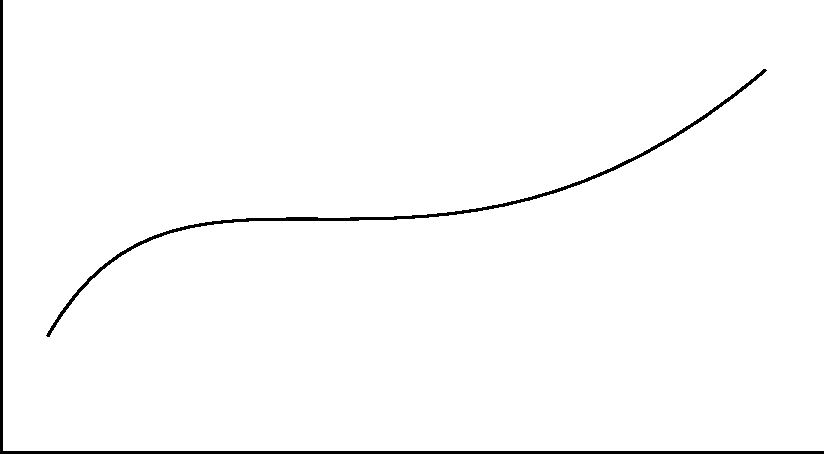
\includegraphics[width=0.7\linewidth]{Figure1}
    \caption{An informative figure.}
    \label{fig:usefulplot}
\end{figure}

\subsection{A sub heading}


\begin{equation}
    \label{eq:beta}
    J = J_0 e^{-\beta d}
\end{equation}



\section{Conclusions}

Some conclusions.

\section{Experimental}
Do not forget to use the SI units package in the experimental.

\section{Acknowledgements}

R.C.C. acknowledges some funding.

\clearpage
\printbibliography

\end{document}
